% ============================================================================
% AD7031 Week 9 -- LECTURE NOTE, version WITH PROOFS (CVaR proposition, VaR <=> chance constraint)
% The classroom version OUU_week09_note.tex omits the two proofs.
%
% Straight conversion of the course folder's handwritten notes:
%   "OUU Lecture 3" p.2 (bottom) - p.4 : optimization under uncertainty, examples
%        (portfolio, shortest path), competing paradigms, stochastic optimization,
%        risk measure, stochastic program, risk neutral, mean-variance
%   "OUU Lecture 4" p.1 - p.4 : Markowitz mean-variance as a convex QP, limits of
%        mean-variance (two pictures), VaR, CVaR, proposition CVaR = E[Z | Z >= VaR]
%        for continuous Z, proof via the derivative in beta
%   "OUU Lecture 5" p.1 - p.3 : proof finished (indicator, conditional expectation),
%        discrete example (atoms at -1, 0, 1; atom splitting), uncertainty in the
%        constraint: E / VaR / CVaR constraints, chance constraint, proposition
%        VaR constraint <=> chance constraint
% Robust optimization and DRO (Lecture 5 p.3 bottom - p.4) are left for weeks 12-13;
% the "competing paradigms" overview stays as a roadmap.
% Changes from the handwritten order: the hand-drawn "same P, different x, different
% loss" sketch (Lecture 3 p.3) is replaced by week09_loss_distribution.pdf, generated
% by loss_distribution_2d.py (two assets, Tech boom/bust vs quiet Energy, Gaussian
% regime mixture; the loss densities are exact 1-D mixtures).  Added at the end:
% the CVaR stochastic program with one beta per risk term, and its scenario LP
% (HW2 Problem 4(d)-(e)).
% Discrete example checked by hand: eps = 1/2, VaR = 0, CVaR = 1/2 (g(beta) = 1/2 + beta/2
% on [0,1], 1/2 - beta/2 on [-1,0]); E[Z | Z >= 0] = 1/3, E[Z | Z > 0] = 1, atom split 1/2.
% Same house style as OUU_week06_note.tex; self-contained -- no \input.
% ============================================================================
\documentclass[10pt]{article}

\usepackage[a4paper, margin=1.9cm]{geometry}
\usepackage{amsmath, amssymb, mathtools}
\usepackage[dvipsnames]{xcolor}
\usepackage{graphicx}
\usepackage{array}
\usepackage{colortbl}
\usepackage{tikz}
\usetikzlibrary{patterns}
\usepackage{dsfont}
\usepackage[hidelinks]{hyperref}

\definecolor{ruleink}{RGB}{18, 68, 140}
\definecolor{demoink}{RGB}{140, 82, 20}
\definecolor{keyink}{RGB}{20, 90, 20}
\definecolor{watchink}{RGB}{86, 60, 140}
\definecolor{punchink}{RGB}{170, 30, 60}
\definecolor{lineA}{RGB}{44, 110, 176}
\definecolor{lineB}{RGB}{168, 96, 32}
\definecolor{lineC}{RGB}{78, 62, 140}

% ---- the pens used in the handwritten original ----------------------------
\definecolor{redink}{RGB}{198, 38, 38}
\definecolor{purpink}{RGB}{132, 58, 176}
\definecolor{grnink}{RGB}{22, 118, 62}
\definecolor{magink}{RGB}{214, 30, 158}
\definecolor{boxink}{RGB}{232, 150, 42}
\definecolor{sandink}{RGB}{250, 206, 142}

\setlength{\parindent}{0pt}
\pagestyle{empty}

% tighter spacing around centered displays
\AtBeginDocument{%
  \abovedisplayskip=7pt plus 2pt
  \belowdisplayskip=7pt plus 2pt
  \abovedisplayshortskip=4pt
  \belowdisplayshortskip=4pt}

% ---- one section -----------------------------------------------------------
\newcommand{\beat}[2]{%   number, title
  \par\bigskip\vspace{4pt}
  {\color{ruleink}\rule{\textwidth}{1pt}}\par\nobreak\vspace{4pt}
  {\large\bfseries #1.\; #2}\par\nobreak\vspace{6pt}}

% ---- board content ---------------------------------------------------------
\newenvironment{board}{%
  \par\vspace{4pt}
  \begingroup\leftskip=1.3em\relax\parskip=2pt\relax}{%
  \par\endgroup\vspace{4pt}}

% ---- hanging bullet (wrapped lines stay indented) --------------------------
\newcommand{\bul}{\hangindent=2.6em\hangafter=1\hspace{1.2em}\textbullet\ \ignorespaces}

% ---- shorthands -------------------------------------------------------------
\newcommand{\R}{\mathcal{R}}
\newcommand{\E}{\mathbb{E}}
\newcommand{\Prob}{\mathbb{P}}
\newcommand{\VaR}{\mathrm{VaR}}
\newcommand{\CVaR}{\mathrm{CVaR}}
\newcommand{\ind}[1]{\mathds{1}_{#1}}
\newcommand{\xit}{\tilde\xi}
\newcommand{\Zt}{\tilde Z}


\begin{document}

{\Large\bfseries Week 9 --- Risk Measures: Mean--Variance, VaR, CVaR}\\[2pt]
{\small AD7031 Optimization Under Uncertainty \quad\textbullet\quad Instructor: Prof.\ H.\ Park \quad\textbullet\quad Oct 24, 2026}

% ---------------------------------------------------------------- 1
\beat{1}{Optimization under uncertainty}
\begin{board}
\textbf{Deterministic optimization}
\vspace{2pt}

\begin{center}
$\begin{aligned}
  \min\quad & f_0(x) \\
  \text{s.t.}\quad & x \in \mathbb{R}^N \\
                   & f_i(x) \le 0 \qquad \forall i \in [I]
\end{aligned}$
\end{center}
\vspace{10pt}

\textbf{OUU:} \quad uncertainty is captured in the vector \ $\xi \in \mathbb{R}^k$
\vspace{4pt}

\quad objective: \ $f_0(x, \xi)$ \qquad constraints: \ $f_i(x, \xi)$ \qquad
$\mathcal{X}$ \ : \ set of \emph{deterministic} constraints on $x$
\vspace{12pt}

\textbf{Examples}
\vspace{4pt}

\quad 1) \textbf{Portfolio optimization:} \quad $\xi$ = vector of asset returns
\vspace{3pt}

\qquad\quad $f_0(x, \xi) = -\xi^{\top}x$ \quad {\color{redink}loss} \qquad\qquad
$\mathcal{X} = \{\, x \in \mathbb{R}^N_+ \;:\; e^{\top}x = W \,\}$
\vspace{2pt}

\qquad\quad {\small ($e$ = all-ones vector, \ $e^{\top}x = x_1 + \cdots + x_N$, \ $W$ = wealth)}
\vspace{8pt}

\quad 2) \textbf{Shortest path:} \quad $\xi$ = vector of edge weights
\vspace{3pt}

\qquad\quad $f_0(x, \xi) = \xi^{\top}x$, \quad $x$ binary vector \qquad\qquad
$\mathcal{X}$ = flow conservation constraints
\vspace{14pt}

\textbf{Competing paradigms for OUU}
\vspace{6pt}

\begin{center}
\begin{tabular}{@{}p{6.4cm}@{\hspace{1.0cm}}p{6.4cm}@{}}
\multicolumn{1}{c}{\fbox{\textbf{Stochastic optimization}}} & \multicolumn{1}{c}{\fbox{\textbf{Robust optimization}}} \\[6pt]
\multicolumn{1}{c}{$\displaystyle \min_{x \in \mathcal{X}} \ \E_{\Prob}\big[\, f_0(x, \xit) \,\big]$} &
\multicolumn{1}{c}{$\displaystyle \min_{x \in \mathcal{X}} \ \mathop{{\color{punchink}\max}}_{\xi \in \Xi} \ f_0(x, \xi)$} \\[8pt]
--- $\xit$ random, with \textbf{known} distribution $\Prob$ &
--- a game against nature: you choose $x$, nature picks the worst $\xi$ in a set $\Xi$ \\
\end{tabular}
\end{center}
\vspace{4pt}

\begin{center}$\searrow$\hspace{2.2cm}$\swarrow$\end{center}
\vspace{-6pt}

\begin{center}
\fbox{\textbf{Distributionally robust optimization}}
\vspace{6pt}

$\displaystyle \min_{x \in \mathcal{X}} \ \mathop{{\color{punchink}\max}}_{\mathbb{Q} \in \mathcal{P}_\lambda(\hat{\Prob}_N)} \ \E_{\mathbb{Q}}\big[\, f_0(x, \xit) \,\big]$
\end{center}
\vspace{2pt}

\quad {\small ${\hat{\Prob}_N}$ = empirical distribution of $N$ samples, \ ${\mathcal{P}_\lambda(\hat{\Prob}_N)}$ = ambiguity set: distributions within distance $\lambda$ of it}
\vspace{4pt}

\quad --- more realistic: don't assume a distribution $\Prob$; only the data $\hat{\Prob}_N$
\vspace{2pt}

\quad --- less conservative: the worst-case \emph{distribution} $\mathbb{Q}$ rather than the worst-case \emph{scenario} $\xi$
\vspace{8pt}

\end{board}

\newpage

% ---------------------------------------------------------------- 2
\beat{2}{Stochastic optimization}
\begin{board}
$\xit \sim \Prob$ \quad random \emph{vector}; \qquad $\Zt = f_0(x, \xit)$ \quad the loss, a univariate random variable
\vspace{6pt}

\quad fix $x$ \ $\Rightarrow$ \ $\Zt$ has a distribution; \qquad change $x$ \ $\Rightarrow$ \ it changes --- \textbf{the decision shapes the distribution}
\vspace{8pt}

\textbf{Example (Portfolio optimization)}
\vspace{2pt}

\begin{center}
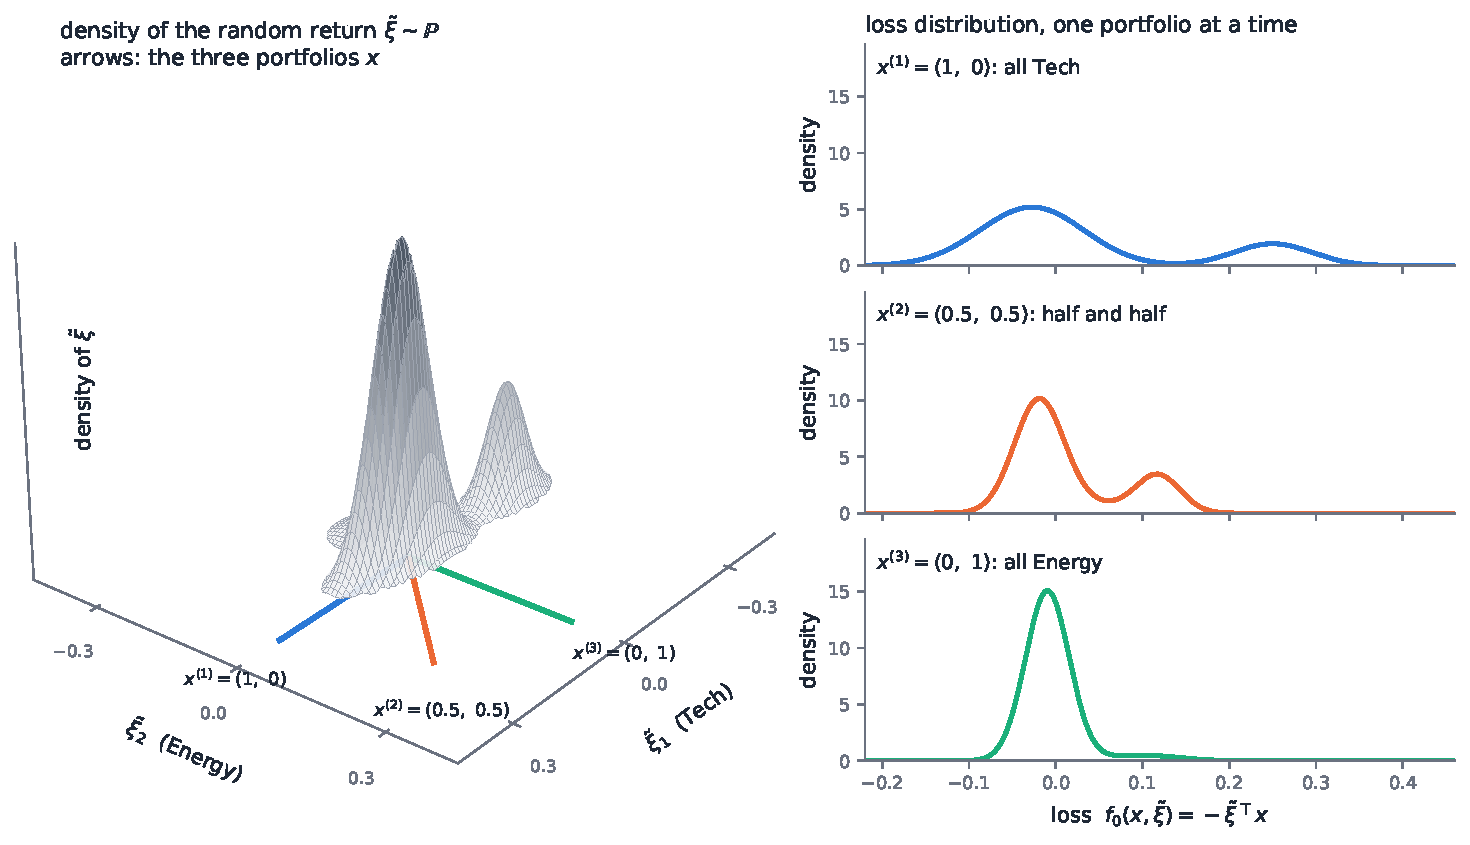
\includegraphics[width=0.78\textwidth]{week09_loss_distribution.pdf}
\end{center}
\vspace{0pt}

\quad two assets, Tech (boom/bust) and Energy (quiet); \ same $\Prob$ on the left, three portfolios on the right
\vspace{3pt}

\quad {\color{punchink}how do we compare the three? \ we need one number per distribution.}
\vspace{8pt}

\textbf{Def (risk measure)} \qquad
$\R_{\Prob} : \mathcal{L} \longrightarrow \mathbb{R}$
\qquad {\small $\mathcal{L}$ = all univariate random variables, \ \ $\mathbb{R}$ = real numbers}
\vspace{10pt}

\textbf{Stochastic program}
\vspace{2pt}

\begin{center}
\fbox{\rule{0pt}{1em}\;
$\begin{aligned}
  \min\quad & \R_{\Prob}\big[f_0(x, \xit)\big] \\
  \text{s.t.}\quad & x \in \mathcal{X} \\
                   & \R_{\Prob}\big[f_i(x, \xit)\big] \le 0 \qquad \forall i \in [I]
\end{aligned}$
\;\rule[-2.6em]{0pt}{1em}}
\hspace{2.5cm} (SP)
\end{center}
\vspace{4pt}

\quad the index $\Prob$ is the distribution of $\xit$: \ every risk measure depends on it
\vspace{8pt}

\textbf{Examples of risk measures}
\vspace{3pt}

\fbox{Risk neutral} \qquad $\R_{\Prob} = \E_{\Prob}$ \ : \ expected value
\vspace{2pt}

\begin{center}
$\begin{aligned}
  \min\quad & \E_{\Prob}\big[f_0(x, \xit)\big] \\
  \text{s.t.}\quad & x \in \mathcal{X} \\
                   & \E_{\Prob}\big[f_i(x, \xit)\big] \le 0 \qquad \forall i \in [I]
\end{aligned}$
\end{center}
\vspace{2pt}

\begin{center}
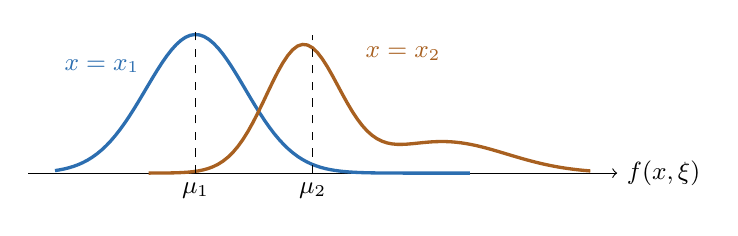
\begin{tikzpicture}[font=\small, x=0.85cm, y=0.8cm]
  \draw[->] (-0.2,0) -- (8.6,0) node[right] {$f(x, \xi)$};
  \draw[very thick, lineA, domain=0.2:6.4, samples=90] plot (\x, {2.2*exp(-(\x-2.3)^2/1.1)});
  \draw[very thick, lineB, domain=1.6:8.2, samples=90] plot (\x, {2.0*exp(-(\x-3.9)^2/0.6) + 0.5*exp(-(\x-6.0)^2/1.8)});
  \draw[dashed] (2.3,0) -- (2.3,2.3);
  \draw[dashed] (4.05,0) -- (4.05,2.2);
  \node[below] at (2.3,0) {$\mu_1$};
  \node[below] at (4.05,0) {$\mu_2$};
  \node[lineA] at (0.9,1.7) {$x = x_1$};
  \node[lineB] at (5.4,1.9) {$x = x_2$};
\end{tikzpicture}
\end{center}
\vspace{2pt}

\quad {\color{redink}$\mu_1 = \E_{\Prob}[f_0(x_1, \xit)] \;<\; \mu_2 = \E_{\Prob}[f_0(x_2, \xit)]$}
\quad $\Rightarrow$ \ $x_1$ is preferable under the risk-neutral measure.
\end{board}

\newpage

% ---------------------------------------------------------------- 3
\beat{3}{Risk averse 1: mean--variance}
\begin{board}
\fbox{Risk averse} \quad 1) \ \textbf{mean--variance} \quad $\R_{\Prob} = \lambda\,\mathrm{Var}_{\Prob} + (1-\lambda)\,\E_{\Prob}$ \ : \ convex combination of mean and variance
\vspace{2pt}

\begin{center}
$\displaystyle \min\ \ \lambda\,\mathrm{Var}_{\Prob}\big[f_0(x, \xit)\big] + (1 - \lambda)\,\E_{\Prob}\big[f_0(x, \xit)\big]$
\qquad {\color{redink}$\lambda \in [0, 1]$}
\end{center}
\vspace{8pt}

\textbf{Example: mean--variance portfolio optimization} \quad (Harry Markowitz, 1952)
\vspace{2pt}

\quad $\xit \in \mathbb{R}^N$ is the vector of asset returns. \quad Assume we know
\vspace{3pt}

\qquad $\E_{\Prob}[\xit] = \mu$ \quad {\color{redink}vector of means}, \qquad
$\E_{\Prob}\big[(\xit - \mu)(\xit - \mu)^{\top}\big] = \E_{\Prob}[\xit\xit^{\top}] - \mu\mu^{\top} = \Sigma$ \quad {\color{redink}covariance matrix}
\vspace{6pt}

\quad an investor allocates a wealth of $\$1$ to minimize the mean--variance of the portfolio loss $-\xit^{\top}x$:
\vspace{4pt}

\begin{center}
\fbox{\rule{0pt}{1em}\;
$\begin{aligned}
  \min\quad & \lambda\,\mathrm{Var}_{\Prob}\big(-\xit^{\top}x\big) + (1-\lambda)\,\E_{\Prob}\big[-\xit^{\top}x\big] \\
  \text{s.t.}\quad & x \in \mathbb{R}^N_+ \\
                   & e^{\top}x = 1
\end{aligned}$
\;\rule[-2.6em]{0pt}{1em}}
\end{center}
\vspace{8pt}

\textbf{reformulate} --- both terms are functions of $\mu$ and $\Sigma$ only:
\vspace{4pt}

\quad $\E_{\Prob}[-\xit^{\top}x] = -\mu^{\top}x$ \qquad {\color{redink}linearity of expectation}
\vspace{6pt}

\quad $\begin{aligned}[t]
  \mathrm{Var}_{\Prob}(-\xit^{\top}x) = \mathrm{Var}_{\Prob}(\xit^{\top}x)
    &= \E_{\Prob}\big[(\xit^{\top}x)^2\big] - \big(\E_{\Prob}[\xit^{\top}x]\big)^2 \\
    &= \E_{\Prob}\big[x^{\top}\xit\xit^{\top}x\big] - (\mu^{\top}x)^2
     = x^{\top}\E_{\Prob}[\xit\xit^{\top}]\,x - x^{\top}\mu\mu^{\top}x \\
    &= x^{\top}\big(\E_{\Prob}[\xit\xit^{\top}] - \mu\mu^{\top}\big)x \\
    &= x^{\top}\Sigma\,x
\end{aligned}$
\vspace{8pt}

\begin{center}
\fbox{\rule{0pt}{1em}\;
$\begin{aligned}
  \min\quad & \lambda\,x^{\top}\Sigma\,x - (1-\lambda)\,\mu^{\top}x \\
  \text{s.t.}\quad & x \in \mathbb{R}^N_+ \\
                   & e^{\top}x = 1
\end{aligned}$
\;\rule[-2.6em]{0pt}{1em}}
\qquad {\color{redink}$\Sigma \succeq 0$ \ $\Rightarrow$ \ convex quadratic program}
\end{center}
\vspace{6pt}

\textbf{Limits of mean--variance}
\vspace{4pt}

\bul for a general loss $f_0(x, \xit)$, \ $\mathrm{Var}_{\Prob}[f_0(x, \xit)]$ need not be convex in $x$ \ --- the mean--variance
risk measure in general leads to a non-convex optimization problem. \ (linear loss: convex, as above)
\vspace{6pt}

\bul variance penalizes spread in \emph{both} directions --- it does not see where the big losses are:
\vspace{4pt}

\begin{center}
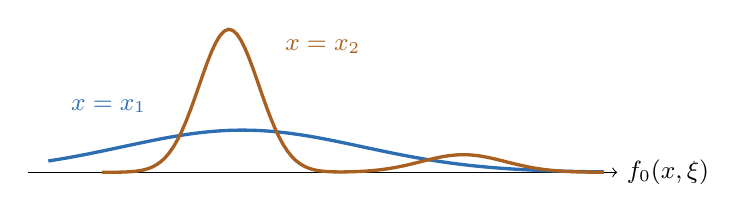
\begin{tikzpicture}[font=\small, x=0.85cm, y=0.8cm]
  % equal mass; x1 ~ N(3.0, 3.2): Var 3.2;  x2 = 0.85 N(2.8, 0.2) + 0.15 N(6.3, 0.4): Var 1.79
  \draw[->] (-0.2,0) -- (8.6,0) node[right] {$f_0(x, \xi)$};
  \draw[very thick, lineA, domain=0.1:8.4, samples=120] plot (\x, {0.67*exp(-(\x-3.0)^2/6.4)});
  \draw[very thick, lineB, domain=0.9:8.4, samples=120] plot (\x, {2.27*exp(-(\x-2.8)^2/0.4) + 0.28*exp(-(\x-6.3)^2/0.8)});
  \node[lineA] at (1.0,1.05) {$x = x_1$};
  \node[lineB] at (4.2,2.0) {$x = x_2$};
\end{tikzpicture}
\end{center}
\vspace{-2pt}

\qquad $x_2$ has lower variance, but has higher probability of generating bigger losses.
\vspace{4pt}

\begin{center}
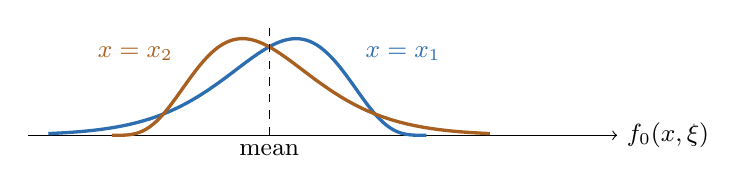
\begin{tikzpicture}[font=\small, x=0.85cm, y=0.8cm]
  % mirror images about the mean 3.4: same mean, same variance.  Gamma(k=6, theta=0.4) shape, unimodal,
  % mildly skewed; x2 = 1.0 + Gamma (tail toward large losses), x1 = 5.8 - Gamma (tail toward small losses)
  \draw[->] (-0.2,0) -- (8.6,0) node[right] {$f_0(x, \xi)$};
  \draw[very thick, lineA, domain=0.1:5.75, samples=140] plot (\x, {0.0729*exp(5*ln((5.8-\x)/0.4) - (5.8-\x)/0.4)});
  \draw[very thick, lineB, domain=1.05:6.7, samples=140] plot (\x, {0.0729*exp(5*ln((\x-1.0)/0.4) - (\x-1.0)/0.4)});
  \draw[dashed] (3.4,0) -- (3.4,1.7);
  \node[below] at (3.4,0) {mean};
  \node[lineA] at (5.4,1.3) {$x = x_1$};
  \node[lineB] at (1.4,1.3) {$x = x_2$};
\end{tikzpicture}
\end{center}
\vspace{-2pt}

\qquad $x_1$ and $x_2$ have the same mean and the same variance (mirror images), so mean--variance cannot tell
them apart; \ but $x_1$ is preferred because it has higher probability of generating smaller losses.
\end{board}

\newpage

% ---------------------------------------------------------------- 4
\beat{4}{Risk averse 2: Value at Risk (VaR)}
\begin{board}
2) \ \textbf{Value at Risk} \quad $\R_{\Prob} = \VaR_{\varepsilon}$ \ : \ $(1 - \varepsilon)$-quantile of the loss
\quad {\color{redink}typically a non-convex optimization problem}
\vspace{3pt}

\quad {\small Of course, $\VaR_{\varepsilon}$ depends on $\Prob$ just like $\E_{\Prob}$ and $\mathrm{Var}_{\Prob}$; \ we omit the index for notational simplicity.}
\vspace{6pt}

\begin{center}
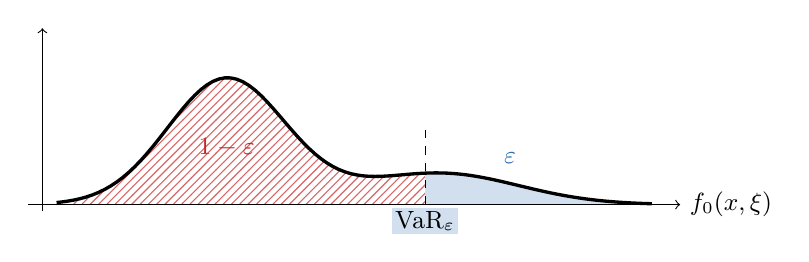
\begin{tikzpicture}[font=\small, x=0.9cm, y=0.8cm]
  % density g = 2.0 N-bump(2.6, 1.4) + 0.5 N-bump(5.6, 2.5);  VaR at 5.4 cuts off eps = 0.14 of the mass
  \fill[pattern=north east lines, pattern color=redink!70]
    (0.4,0) -- plot[domain=0.4:5.4, samples=70] (\x, {2.0*exp(-(\x-2.6)^2/1.4) + 0.5*exp(-(\x-5.6)^2/2.5)}) -- (5.4,0) -- cycle;
  \fill[lineA!22]
    (5.4,0) -- plot[domain=5.4:8.6, samples=60] (\x, {2.0*exp(-(\x-2.6)^2/1.4) + 0.5*exp(-(\x-5.6)^2/2.5)}) -- (8.6,0) -- cycle;
  \draw[->] (-0.2,0) -- (9.0,0) node[right] {$f_0(x, \xi)$};
  \draw[->] (0,-0.1) -- (0,2.8);
  \draw[very thick, black, domain=0.2:8.6, samples=100] plot (\x, {2.0*exp(-(\x-2.6)^2/1.4) + 0.5*exp(-(\x-5.6)^2/2.5)});
  \node[redink] at (2.6,0.9) {$1 - \varepsilon$};
  \draw[dashed] (5.4,0) -- (5.4,1.2);
  \node[lineA, above] at (6.6,0.5) {$\varepsilon$};
  \node[below, fill=lineA!22, inner sep=1pt] at (5.4,-0.05) {$\VaR_{\varepsilon}$};
\end{tikzpicture}
\end{center}
\vspace{2pt}

\quad --- popular in finance
\vspace{2pt}

\quad --- imposed by the Basel II accord: how much capital banks need to set aside to hold against financial risks
\vspace{12pt}

\textbf{Formally:}
\vspace{2pt}

\begin{center}
$\begin{aligned}
  \VaR_{\varepsilon}\big[f_0(x, \xit)\big] \;=\; \min\quad & t \\
  \text{s.t.}\quad & \Prob\big(f_0(x, \xit) \le t\big) \ge 1 - \varepsilon
\end{aligned}$
\hspace{1.2cm}{\color{redink}$\leftarrow$ chance / probability constraint}
\end{center}
\vspace{2pt}

\hspace{7.2cm}{\color{redink}generally non-convex, highly intractable}
\vspace{6pt}

\quad the smallest loss level $t$ that is exceeded with probability at most $\varepsilon$
\vspace{4pt}

\quad VaR risk measure in general leads to a non-convex optimization problem.
\end{board}

% ---------------------------------------------------------------- 5
\beat{5}{Risk averse 3: Conditional Value at Risk (CVaR)}
\begin{board}
3) \ \textbf{Conditional Value at Risk} \quad $\R_{\Prob} = \CVaR_{\varepsilon}$ \ : \ average loss in the worst $\varepsilon$ fraction of outcomes
\quad {\color{redink}(Rockafellar \& Uryasev, 2000)}
\vspace{3pt}

\quad --- CVaR leads to a \textbf{convex} optimization problem if \ $f(x, \xi)$ \ is convex in $x$
\vspace{2pt}

\quad --- imposed by the Basel III accord
\vspace{6pt}

\begin{center}
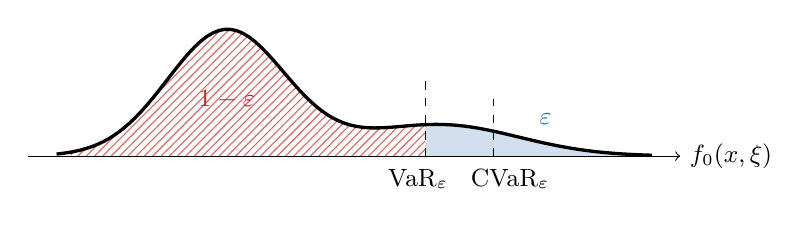
\begin{tikzpicture}[font=\small, x=0.9cm, y=0.8cm]
  % same density and VaR as the VaR picture;  CVaR = conditional mean of the tail beyond VaR = 6.37
  \fill[pattern=north east lines, pattern color=redink!70]
    (0.4,0) -- plot[domain=0.4:5.4, samples=70] (\x, {2.0*exp(-(\x-2.6)^2/1.4) + 0.5*exp(-(\x-5.6)^2/2.5)}) -- (5.4,0) -- cycle;
  \fill[lineA!22]
    (5.4,0) -- plot[domain=5.4:8.6, samples=60] (\x, {2.0*exp(-(\x-2.6)^2/1.4) + 0.5*exp(-(\x-5.6)^2/2.5)}) -- (8.6,0) -- cycle;
  \draw[->] (-0.2,0) -- (9.0,0) node[right] {$f_0(x, \xi)$};
  \draw[very thick, black, domain=0.2:8.6, samples=100] plot (\x, {2.0*exp(-(\x-2.6)^2/1.4) + 0.5*exp(-(\x-5.6)^2/2.5)});
  \node[redink] at (2.6,0.9) {$1 - \varepsilon$};
  \draw[dashed] (5.4,0) -- (5.4,1.2);
  \draw[dashed] (6.37,0) -- (6.37,0.9);
  \node[lineA, above] at (7.1,0.35) {$\varepsilon$};
  \node[below] at (5.3,-0.05) {$\VaR_{\varepsilon}$};
  \node[below] at (6.6,-0.05) {$\CVaR_{\varepsilon}$};
\end{tikzpicture}
\end{center}
\vspace{4pt}

\begin{center}
\fbox{\rule{0pt}{1em}\;
$\displaystyle \CVaR_{\varepsilon}\big[f_0(x, \xit)\big] \;=\; \min_{\beta \in \mathbb{R}}\ \
  \beta + \frac{1}{\varepsilon}\,\E_{\Prob}\Big[\max\big\{f_0(x, \xit) - \beta,\ 0\big\}\Big]$
\;\rule[-1.4em]{0pt}{1em}}
\end{center}
\vspace{4pt}

\quad the objective is convex in $(x, \beta)$ when $f_0$ is convex in $x$: \ $\max\{\text{convex}, 0\}$ is convex,
and $\E$ keeps it convex.
\vspace{10pt}

Recall \ $\Zt = f_0(x, \xit)$.
\vspace{6pt}

\begin{center}
\fbox{\rule{0pt}{1em}\;
\textbf{Proposition:} \ if $\Zt$ has a continuous distribution, then \quad
$\CVaR_{\varepsilon}[\Zt] = \E_{\Prob}\big[\Zt \,\big|\, \Zt \ge \VaR_{\varepsilon}[\Zt]\big]$
\;\rule[-0.6em]{0pt}{1em}}
\end{center}
\vspace{2pt}

\quad --- CVaR = the \textbf{average loss in the worst $\varepsilon$ fraction} of outcomes; \ so \ $\CVaR_{\varepsilon} \ge \VaR_{\varepsilon}$.
\vspace{8pt}

\newpage
\textbf{Proof:} \quad step 1 --- find the minimizer $\beta^{*}$.
\vspace{3pt}

\quad $\displaystyle \frac{\partial}{\partial\beta}\Big(\beta + \frac{1}{\varepsilon}\,\E_{\Prob}\big[\max\{\Zt - \beta, 0\}\big]\Big) = 0$
\vspace{3pt}

\quad $\displaystyle 1 + \frac{1}{\varepsilon}\,\E_{\Prob}\Big[\frac{\partial}{\partial\beta}\max\{\Zt - \beta, 0\}\Big] = 0$
\hspace{1.5cm}
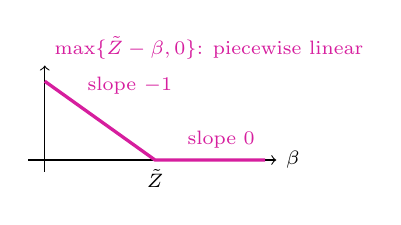
\begin{tikzpicture}[baseline=0.4cm, font=\scriptsize, x=0.7cm, y=0.5cm]
  \draw[->] (-0.3,0) -- (4.2,0) node[right] {$\beta$};
  \draw[->] (0,-0.3) -- (0,2.4);
  \draw[very thick, magink] (0,2.0) -- (2.0,0) -- (4.0,0);
  \node[below] at (2.0,0) {$\Zt$};
  \node[magink, right] at (0.6,1.9) {slope $-1$};
  \node[magink, above] at (3.2,0.05) {slope $0$};
  \node[magink, above right] at (0,2.3) {$\max\{\Zt - \beta, 0\}$: piecewise linear};
\end{tikzpicture}
\vspace{3pt}

\quad $\displaystyle 1 + \frac{1}{\varepsilon}\,\E_{\Prob}\big[-\ind{\Zt > \beta}\big] = 0$
\hspace{2.2cm}{\color{redink}indicator function: \ $\ind{A} = \begin{cases} 1 & \text{if } A \text{ holds} \\ 0 & \text{otherwise}\end{cases}$}
\vspace{3pt}

\quad $\displaystyle 1 - \frac{1}{\varepsilon}\,\Prob(\Zt > \beta) = 0$
\hspace{3.3cm}{\color{redink}$\E_{\Prob}[\ind{A}] = \Prob(A)$}
\vspace{3pt}

\quad $\Prob(\Zt > \beta) = \varepsilon$ \qquad $\Rightarrow$ \qquad {\color{purpink}$\beta^{*} = \VaR_{\varepsilon}[\Zt]$}
\vspace{5pt}

\quad step 2 --- plug $\beta^{*}$ in. \quad Since $\Zt$ is continuous, \ $\Prob(\Zt \ge \beta^{*}) = \Prob(\Zt > \beta^{*}) = \varepsilon$:
\vspace{3pt}

\quad $\begin{aligned}[t]
  \CVaR_{\varepsilon}[\Zt]
    &= \beta^{*} + \frac{1}{\varepsilon}\,\E_{\Prob}\big[\max\{\Zt - \beta^{*}, 0\}\big] \\
    &= \beta^{*} + \frac{1}{\varepsilon}\,\E_{\Prob}\big[(\Zt - \beta^{*})\,\ind{\Zt \ge \beta^{*}}\big] \\
    &= \beta^{*} + \frac{1}{\Prob(\Zt \ge \beta^{*})}\,\E_{\Prob}\big[\Zt\,\ind{\Zt \ge \beta^{*}}\big]
       - \frac{1}{\Prob(\Zt \ge \beta^{*})}\,\E_{\Prob}\big[\beta^{*}\,\ind{\Zt \ge \beta^{*}}\big] \\
    &= \beta^{*} + \E_{\Prob}\big[\Zt \,\big|\, \Zt \ge \beta^{*}\big] - \beta^{*} \\
    &= \E_{\Prob}\big[\Zt \,\big|\, \Zt \ge \VaR_{\varepsilon}[\Zt]\big] \qquad \blacksquare
\end{aligned}$
\vspace{5pt}

\begin{center}
\fbox{\rule{0pt}{1em}\;
\textbf{Def (conditional expectation)} \qquad
$\displaystyle \E_{\Prob}\big[\Zt \,\big|\, \Zt \in A\big] = \frac{\E_{\Prob}\big[\Zt\,\ind{\Zt \in A}\big]}{\Prob(\Zt \in A)}$
\;\rule[-1.3em]{0pt}{1em}}
\end{center}
\end{board}

\begin{board}
\textbf{$\Zt$ has a discrete distribution} --- what does the proposition become?
\vspace{4pt}

\quad Consider: \ $\Prob(\Zt = 1) = \tfrac14$, \quad $\Prob(\Zt = 0) = \tfrac12$, \quad $\Prob(\Zt = -1) = \tfrac14$.
\qquad Let \ $\varepsilon = \tfrac12$.
\hspace{1.0cm}
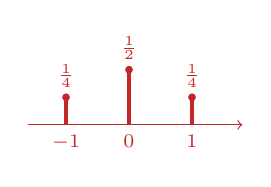
\begin{tikzpicture}[baseline=0.1cm, font=\scriptsize, x=0.8cm, y=1.4cm]
  \draw[->, redink] (-1.6,0) -- (1.8,0);
  \foreach \p/\h in {-1/0.25, 0/0.5, 1/0.25} {
    \draw[very thick, redink] (\p,0) -- (\p,\h);
    \fill[redink] (\p,\h) circle (1.4pt);
    \node[below, redink] at (\p,0) {$\p$};
  }
  \node[redink, above] at (-1,0.25) {$\tfrac14$};
  \node[redink, above] at (0,0.5) {$\tfrac12$};
  \node[redink, above] at (1,0.25) {$\tfrac14$};
\end{tikzpicture}
\vspace{4pt}

\quad $\begin{aligned}[t]
  \VaR_{\varepsilon}[\Zt] = \min_{t \in \mathbb{R}}\ \ & t \\
  \text{s.t.}\ \ & \Prob(\Zt \le t) \ge 1 - \tfrac12
\end{aligned}$
\quad $= 0$ \qquad {\small ($\Prob(\Zt \le 0) = \tfrac34 \ge \tfrac12$, \ and for any $t < 0$, \ $\Prob(\Zt \le t) \le \tfrac14$)}
\vspace{5pt}

\quad $\begin{aligned}[t]
  \CVaR_{\varepsilon}[\Zt]
    &= \min_{\beta \in \mathbb{R}}\ \beta + \frac{1}{\varepsilon}\,\E_{\Prob}\big[\max\{\Zt - \beta, 0\}\big] \\
    &= \min_{\beta \in \mathbb{R}}\ \beta + \frac{1}{1/2}\Big( \tfrac14 \max\{1 - \beta, 0\}
       + \tfrac12 \max\{0 - \beta, 0\} + \tfrac14 \max\{-1 - \beta, 0\} \Big) \\
    &= \tfrac12 \qquad {\small \text{(attained at } \beta = 0\text{: the objective is } \tfrac12 + \tfrac{\beta}{2} \text{ on } [0,1]
       \text{ and } \tfrac12 - \tfrac{\beta}{2} \text{ on } [-1, 0])}
\end{aligned}$
\vspace{5pt}

\quad but \quad $\displaystyle \E_{\Prob}\big[\Zt \,\big|\, \Zt \ge \underbrace{\VaR_{\varepsilon}[\Zt]}_{0}\big]
  = \frac{\tfrac12 \times 0 + \tfrac14 \times 1}{\tfrac12 + \tfrac14} = \tfrac13$
\qquad and \qquad
$\displaystyle \E_{\Prob}\big[\Zt \,\big|\, \Zt > \VaR_{\varepsilon}[\Zt]\big] = \frac{\tfrac14 \times 1}{\tfrac14} = 1$
\vspace{4pt}

\quad neither is $\tfrac12$: \ the atom at $\VaR_{\varepsilon}$ is too big --- $\Prob(\Zt \ge 0) = \tfrac34 > \varepsilon$ but $\Prob(\Zt > 0) = \tfrac14 < \varepsilon$.
\vspace{5pt}

\textbf{Atom splitting} \quad split the atom at $0$ so that exactly $\varepsilon = \tfrac12$ of the mass lies in the tail:
\hspace{0.8cm}
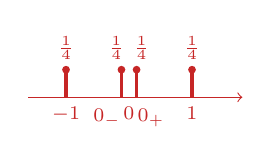
\begin{tikzpicture}[baseline=0.1cm, font=\scriptsize, x=0.8cm, y=1.4cm]
  \draw[->, redink] (-1.6,0) -- (1.8,0);
  \foreach \p/\h in {-1/0.25, -0.12/0.25, 0.12/0.25, 1/0.25} {
    \draw[very thick, redink] (\p,0) -- (\p,\h);
    \fill[redink] (\p,\h) circle (1.4pt);
  }
  \node[below, redink] at (-1,0) {$-1$}; \node[below, redink] at (0,0) {$0$}; \node[below, redink] at (1,0) {$1$};
  \node[redink, above] at (-1,0.25) {$\tfrac14$}; \node[redink, above] at (-0.2,0.25) {$\tfrac14$};
  \node[redink, above] at (0.2,0.25) {$\tfrac14$}; \node[redink, above] at (1,0.25) {$\tfrac14$};
  \node[redink, below] at (-0.35,-0.02) {$0_-$}; \node[redink, below] at (0.35,-0.02) {$0_+$};
\end{tikzpicture}
\vspace{4pt}

\quad $\displaystyle \E_{\Prob}\big[\Zt \,\big|\, \Zt \ge 0_+\big] = \frac{\tfrac14 \times 0 + \tfrac14 \times 1}{\tfrac12} = \tfrac12$
\qquad $= \CVaR_{\varepsilon}[\Zt]$ \quad $\checkmark$
\vspace{4pt}

\quad {\color{keyink}in general: CVaR = the average of the worst $\varepsilon$ of the probability mass, with the atom at $\VaR_{\varepsilon}$ split
as needed. \ The $\min_{\beta}$ formula gets this right automatically.}
\end{board}

% ---------------------------------------------------------------- 6
\beat{6}{Uncertainty in the constraint}
\begin{board}
How to handle uncertainty in the constraint? \qquad $\R_{\Prob}\big[f_i(x, \xit)\big] \le 0$
\vspace{4pt}

\quad --- $\E_{\Prob}\big[f_i(x, \xit)\big] \le 0$ \qquad\qquad the constraint holds \emph{on average}
\vspace{3pt}

\quad --- $\VaR_{\varepsilon}\big[f_i(x, \xit)\big] \le 0$
\qquad {\color{redink}non-convex in general}
\vspace{3pt}

\qquad $\displaystyle \iff\ \min_{t \in \mathbb{R}}\big\{\, t \;:\; \Prob\big(f_i(x, \xit) \le t\big) \ge 1 - \varepsilon \,\big\} \le 0$
\vspace{3pt}

\qquad $\displaystyle \iff\ \exists\, t \le 0 \;:\; \Prob\big(f_i(x, \xit) \le t\big) \ge 1 - \varepsilon$
\vspace{3pt}

\qquad $\displaystyle \iff\ \Prob\big(f_i(x, \xit) \le 0\big) \ge 1 - \varepsilon$
\vspace{3pt}

\quad --- $\CVaR_{\varepsilon}\big[f_i(x, \xit)\big] \le 0$
\qquad {\color{redink}convex; gives an upper bound on $\VaR_{\varepsilon}$, so it implies the VaR constraint}
\vspace{3pt}

\qquad $\displaystyle \iff\ \min_{\beta}\ \beta + \frac{1}{\varepsilon}\,\E_{\Prob}\big[\max\{f_i(x, \xit) - \beta, 0\}\big] \le 0$
\vspace{3pt}

\qquad $\displaystyle \iff\ \exists\, \beta \in \mathbb{R} \;:\; \beta + \frac{1}{\varepsilon}\,\E_{\Prob}\big[\max\{f_i(x, \xit) - \beta, 0\}\big] \le 0$
\vspace{4pt}

\textbf{Chance constraint / probabilistic constraint} \qquad
$\Prob\big(f_i(x, \xit) \le 0\big) \ge 1 - \varepsilon$
\vspace{5pt}

\begin{center}
\fbox{\rule{0pt}{1em}\;
\textbf{Proposition:} \quad $\VaR_{\varepsilon}$ constraint \ $\iff$ \ chance constraint
\;\rule[-0.6em]{0pt}{1em}}
\end{center}
\vspace{4pt}

\textbf{Putting it together --- the CVaR stochastic program}
\vspace{2pt}

\quad one $\beta$ per risk term: \ $\beta_0$ for the objective, $\beta_i$ for constraint $i$; \ all of them join the outer $\min$
\vspace{4pt}

\begin{center}
$\begin{aligned}
  \min_{x \in \mathcal{X},\ \beta_0, \dots, \beta_I \in \mathbb{R}}\quad
    & \beta_0 + \frac{1}{\varepsilon}\,\E_{\Prob}\Big[\max\big\{f_0(x, \xit) - \beta_0,\ 0\big\}\Big] \\
  \text{s.t.}\quad
    & \beta_i + \frac{1}{\varepsilon}\,\E_{\Prob}\Big[\max\big\{f_i(x, \xit) - \beta_i,\ 0\big\}\Big] \le 0 \qquad \forall i \in [I]
\end{aligned}$
\end{center}
\vspace{4pt}

\quad convex whenever every $f_i$ is convex in $x$.
\vspace{5pt}

\quad \textbf{with $S$ scenarios} \ $\xi^s$ of probabilities $p_s$ \ (i.i.d.\ data: $p_s = \tfrac1S$), \ replace each $\max$ by a variable $u_{is} \ge 0$
\vspace{4pt}

\begin{center}
$\begin{aligned}
  \min\quad & \beta_0 + \frac{1}{\varepsilon}\sum_{s \in [S]} p_s\, u_{0s} \\
  \text{s.t.}\quad & \beta_i + \frac{1}{\varepsilon}\sum_{s \in [S]} p_s\, u_{is} \le 0 && \forall i \in [I] \\
                   & u_{is} \ge f_i(x, \xi^s) - \beta_i, \quad u_{is} \ge 0 && \forall i \in \{0\} \cup [I],\ s \in [S] \\
                   & x \in \mathcal{X}
\end{aligned}$
\end{center}
\vspace{4pt}

\quad {\color{keyink}linear $f_i$ and polyhedral $\mathcal{X}$ \ $\Rightarrow$ \ a linear program. \quad
The same trick on $\VaR_{\varepsilon}$ needs a binary variable per scenario (which scenarios may violate the constraint)
--- a mixed-integer program. \ That is why CVaR is the tractable one.}
\end{board}

\end{document}
